% Options for packages loaded elsewhere
\PassOptionsToPackage{unicode}{hyperref}
\PassOptionsToPackage{hyphens}{url}
%
\documentclass[
  ignorenonframetext,
]{beamer}
\usepackage{pgfpages}
\setbeamertemplate{caption}[numbered]
\setbeamertemplate{caption label separator}{: }
\setbeamercolor{caption name}{fg=normal text.fg}
\beamertemplatenavigationsymbolsempty
% Prevent slide breaks in the middle of a paragraph
\widowpenalties 1 10000
\raggedbottom
\setbeamertemplate{part page}{
  \centering
  \begin{beamercolorbox}[sep=16pt,center]{part title}
    \usebeamerfont{part title}\insertpart\par
  \end{beamercolorbox}
}
\setbeamertemplate{section page}{
  \centering
  \begin{beamercolorbox}[sep=12pt,center]{part title}
    \usebeamerfont{section title}\insertsection\par
  \end{beamercolorbox}
}
\setbeamertemplate{subsection page}{
  \centering
  \begin{beamercolorbox}[sep=8pt,center]{part title}
    \usebeamerfont{subsection title}\insertsubsection\par
  \end{beamercolorbox}
}
\AtBeginPart{
  \frame{\partpage}
}
\AtBeginSection{
  \ifbibliography
  \else
    \frame{\sectionpage}
  \fi
}
\AtBeginSubsection{
  \frame{\subsectionpage}
}
\usepackage{amsmath,amssymb}
\usepackage{lmodern}
\usepackage{iftex}
\ifPDFTeX
  \usepackage[T1]{fontenc}
  \usepackage[utf8]{inputenc}
  \usepackage{textcomp} % provide euro and other symbols
\else % if luatex or xetex
  \usepackage{unicode-math}
  \defaultfontfeatures{Scale=MatchLowercase}
  \defaultfontfeatures[\rmfamily]{Ligatures=TeX,Scale=1}
\fi
\usecolortheme{dove}
\usefonttheme{structurebold}
% Use upquote if available, for straight quotes in verbatim environments
\IfFileExists{upquote.sty}{\usepackage{upquote}}{}
\IfFileExists{microtype.sty}{% use microtype if available
  \usepackage[]{microtype}
  \UseMicrotypeSet[protrusion]{basicmath} % disable protrusion for tt fonts
}{}
\makeatletter
\@ifundefined{KOMAClassName}{% if non-KOMA class
  \IfFileExists{parskip.sty}{%
    \usepackage{parskip}
  }{% else
    \setlength{\parindent}{0pt}
    \setlength{\parskip}{6pt plus 2pt minus 1pt}}
}{% if KOMA class
  \KOMAoptions{parskip=half}}
\makeatother
\usepackage{xcolor}
\IfFileExists{xurl.sty}{\usepackage{xurl}}{} % add URL line breaks if available
\IfFileExists{bookmark.sty}{\usepackage{bookmark}}{\usepackage{hyperref}}
\hypersetup{
  pdftitle={The role of communities of practice for career development in computational statistics},
  pdfauthor={Laura Vana-Gür (TU Wien)},
  hidelinks,
  pdfcreator={LaTeX via pandoc}}
\urlstyle{same} % disable monospaced font for URLs
\newif\ifbibliography
\usepackage{graphicx}
\makeatletter
\def\maxwidth{\ifdim\Gin@nat@width>\linewidth\linewidth\else\Gin@nat@width\fi}
\def\maxheight{\ifdim\Gin@nat@height>\textheight\textheight\else\Gin@nat@height\fi}
\makeatother
% Scale images if necessary, so that they will not overflow the page
% margins by default, and it is still possible to overwrite the defaults
% using explicit options in \includegraphics[width, height, ...]{}
\setkeys{Gin}{width=\maxwidth,height=\maxheight,keepaspectratio}
% Set default figure placement to htbp
\makeatletter
\def\fps@figure{htbp}
\makeatother
\setlength{\emergencystretch}{3em} % prevent overfull lines
\providecommand{\tightlist}{%
  \setlength{\itemsep}{0pt}\setlength{\parskip}{0pt}}
\setcounter{secnumdepth}{-\maxdimen} % remove section numbering
\newlength{\cslhangindent}
\setlength{\cslhangindent}{1.5em}
\newlength{\csllabelwidth}
\setlength{\csllabelwidth}{3em}
\newlength{\cslentryspacingunit} % times entry-spacing
\setlength{\cslentryspacingunit}{\parskip}
\newenvironment{CSLReferences}[2] % #1 hanging-ident, #2 entry spacing
 {% don't indent paragraphs
  \setlength{\parindent}{0pt}
  % turn on hanging indent if param 1 is 1
  \ifodd #1
  \let\oldpar\par
  \def\par{\hangindent=\cslhangindent\oldpar}
  \fi
  % set entry spacing
  \setlength{\parskip}{#2\cslentryspacingunit}
 }%
 {}
\usepackage{calc}
\newcommand{\CSLBlock}[1]{#1\hfill\break}
\newcommand{\CSLLeftMargin}[1]{\parbox[t]{\csllabelwidth}{#1}}
\newcommand{\CSLRightInline}[1]{\parbox[t]{\linewidth - \csllabelwidth}{#1}\break}
\newcommand{\CSLIndent}[1]{\hspace{\cslhangindent}#1}
\usepackage{pifont}
\hypersetup{colorlinks=true, urlcolor=cyan}
\AtBeginEnvironment{CSLReferences}{\tiny}
\setbeamertemplate{itemize items}[circle]
\ifLuaTeX
  \usepackage{selnolig}  % disable illegal ligatures
\fi

\title{The role of communities of practice for career development in
computational statistics}
\subtitle{COMPSTAT 2022, Bologna, Italy}
\author{Laura Vana-Gür (TU Wien)}
\date{2022-08-26}

\begin{document}
\frame{\titlepage}

\begin{frame}{Roadmap}
\protect\hypertarget{roadmap}{}
\begin{itemize}
\item
  Communities of practice (CoPs): what are they? \newline
\item
  Why are CoPs important and how can they be sustained? \newline
\item
  Some CoPs in CompStat and Data Science \newline
\item
  Some guidelines in building inclusive communities and events
\end{itemize}
\end{frame}

\begin{frame}{What are communities of practice? (I)}
\protect\hypertarget{what-are-communities-of-practice-i}{}
\emph{Communities of practice are
\textbf{\textcolor[HTML]{d6d9d9}{groups of people}} who share a
\textbf{\textcolor[HTML]{d4bdba}{concern}} or a
\textbf{\textcolor[HTML]{d4bdba}{passion}} for something they
\textbf{\textcolor[HTML]{edaa98}{do}} and learn how to
\textbf{\textcolor[HTML]{edaa98}{do}} it better as they
\textbf{\textcolor[HTML]{d6d9d9}{interact regularly}}.}
\href{https://wenger-trayner.com/introduction-to-communities-of-practice}{(Wenger-Trayner)}


\includegraphics{figs/3.png}
\end{frame}

\begin{frame}{What are communities of practice? (II)}
\protect\hypertarget{what-are-communities-of-practice-ii}{}
CoPs are characterized by: being informal (typically),\\
voluntary membership, high degree of identification with the group.
(Erik Andriessen 2005; C. Hoadley 2012)

\begin{itemize}
\tightlist
\item
  Examples: group of researchers working on a similar problem who meet
  on a regular basis, meetup groups etc.
\end{itemize}
\end{frame}

\begin{frame}{What are communities of practice? (III)}
\protect\hypertarget{what-are-communities-of-practice-iii}{}
More formally: Concept from social or situated learning theory (Lave and
Wenger 1991; Brown and Duguid 1991; Orr 1990; Constant II 1987)

\begin{itemize}
\item
  CoPs are used to describe the process of learning and the spread of
  knowledge.
\item
  Situated view to learning: \emph{learning is a relational property
  enacted by groups of people in context and in interaction with one
  another} (Lave and Wenger 1991)
\item
  CoPs are groups in which a constant process of legitimate
  \textbf{peripheral participation} takes place (Lave and Wenger 1991).
\end{itemize}
\end{frame}

\begin{frame}{Community composition: Foster inward mobility!}
\protect\hypertarget{community-composition-foster-inward-mobility}{}
\begin{figure}
\centering
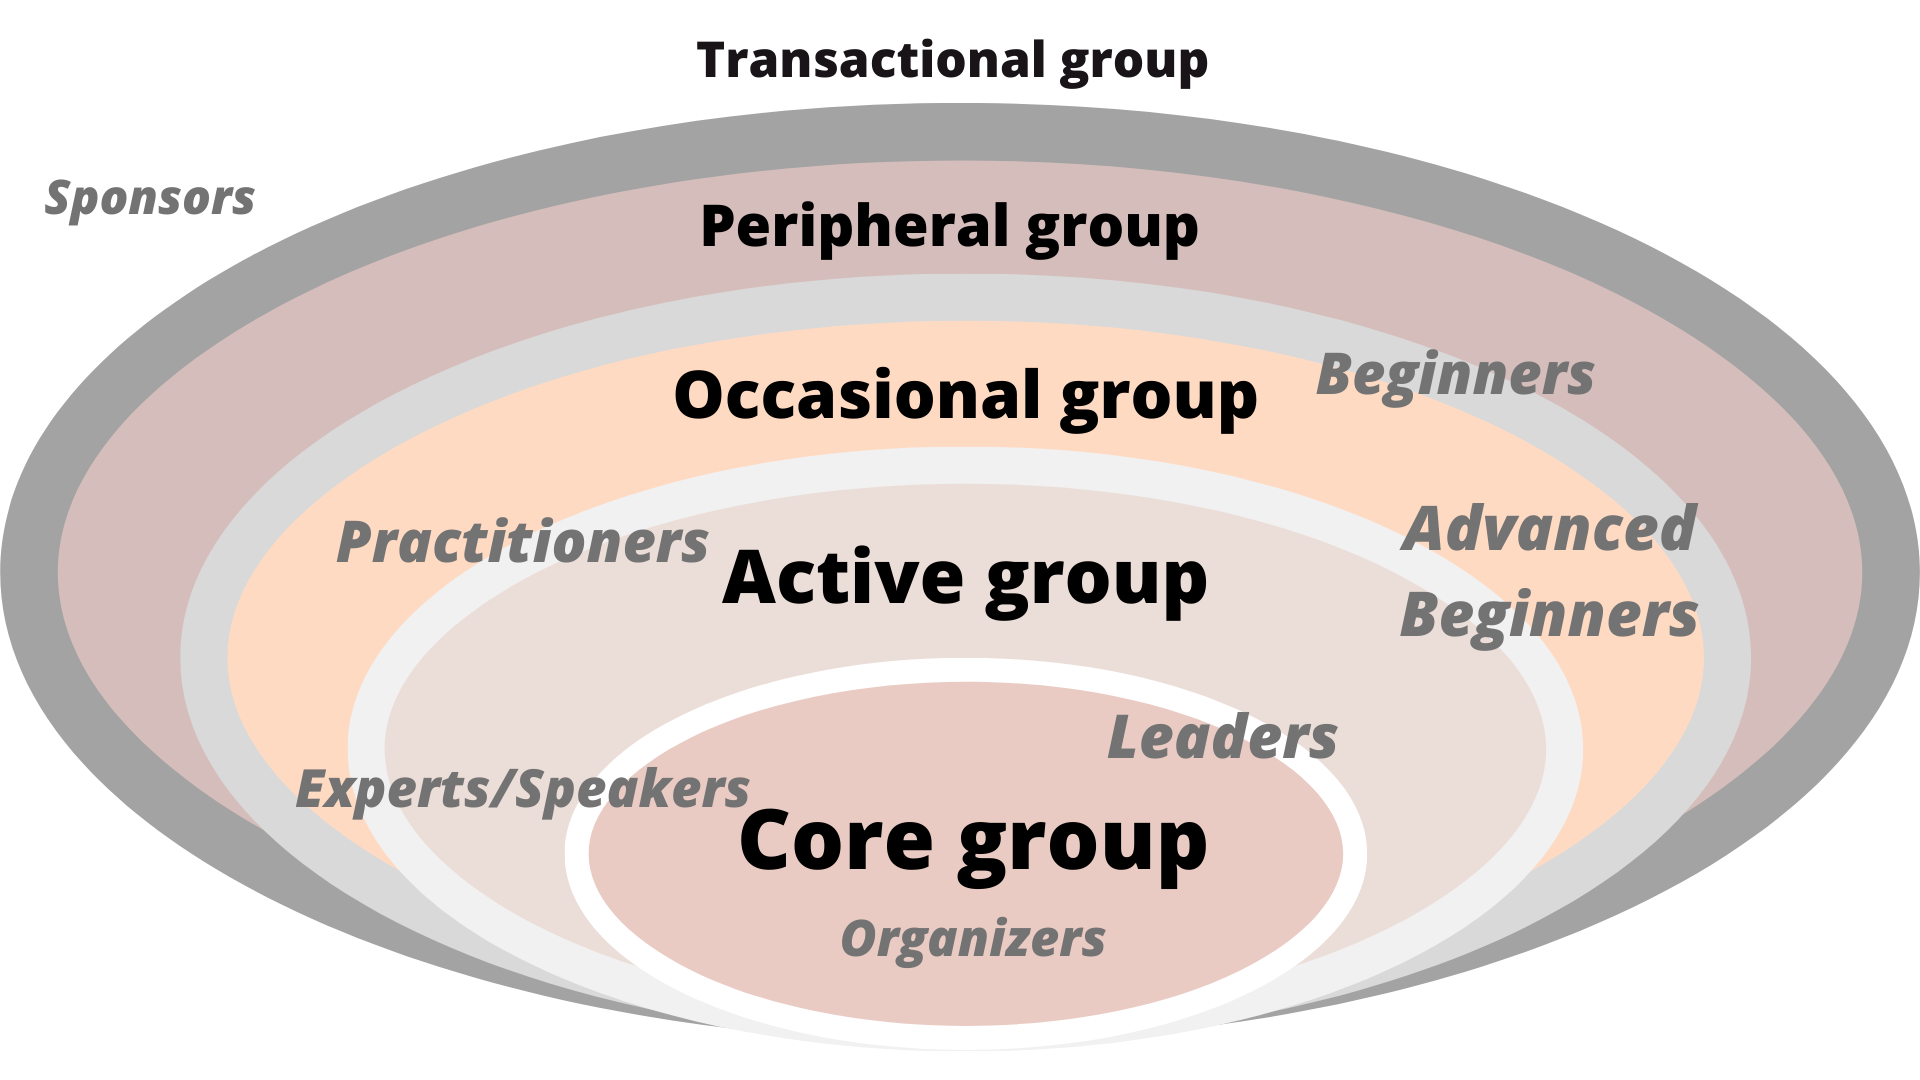
\includegraphics[width=1\textwidth,height=\textheight]{figs/1.png}
\caption{Inspired from
\href{https://wenger-trayner.com/project/levels-of-participation/}{Wenger-Trayner},
Stevens et al. (2018)}
\end{figure}
\end{frame}

\begin{frame}{Goals of CoPs}
\protect\hypertarget{goals-of-cops}{}
(Wenger and Snyder 2000)

\begin{itemize}
\item
  help to solve problems quickly \newline
\item
  develop professional skills \newline
\item
  set and transfer best practices
\end{itemize}
\end{frame}

\begin{frame}{Member benefits}
\protect\hypertarget{member-benefits}{}
(Wenger and Snyder 2000)

\begin{itemize}
\item
  \textbf{short-term}: help with challenges, access to expertise,
  confidence, meaningful work, social aspects \newline
\item
  \textbf{long-term}: personal development, enhanced reputation,
  professional identity, networking
\end{itemize}
\end{frame}

\begin{frame}{Techniques to foster learning-oriented CoPs}
\protect\hypertarget{techniques-to-foster-learning-oriented-cops}{}
\begin{enumerate}
\item
  improve \textbf{connectivity} -- linking people with others who have
  similar practices (social networking, directories or profiles)
\item
  access to \textbf{content} -- shared repository of information that is
  used by the community in its practices
\item
  supporting \textbf{conversation} -- providing tools for discussing
  with others in the community
\item
  providing information \textbf{context} -- providing awareness of the
  information context of various resources
\end{enumerate}

based on the C4P model in Kilner (2004) and C. M. Hoadley and Kilner
(2005)
\end{frame}

\begin{frame}{CoPs in CompStat and data science}
\protect\hypertarget{cops-in-compstat-and-data-science}{}
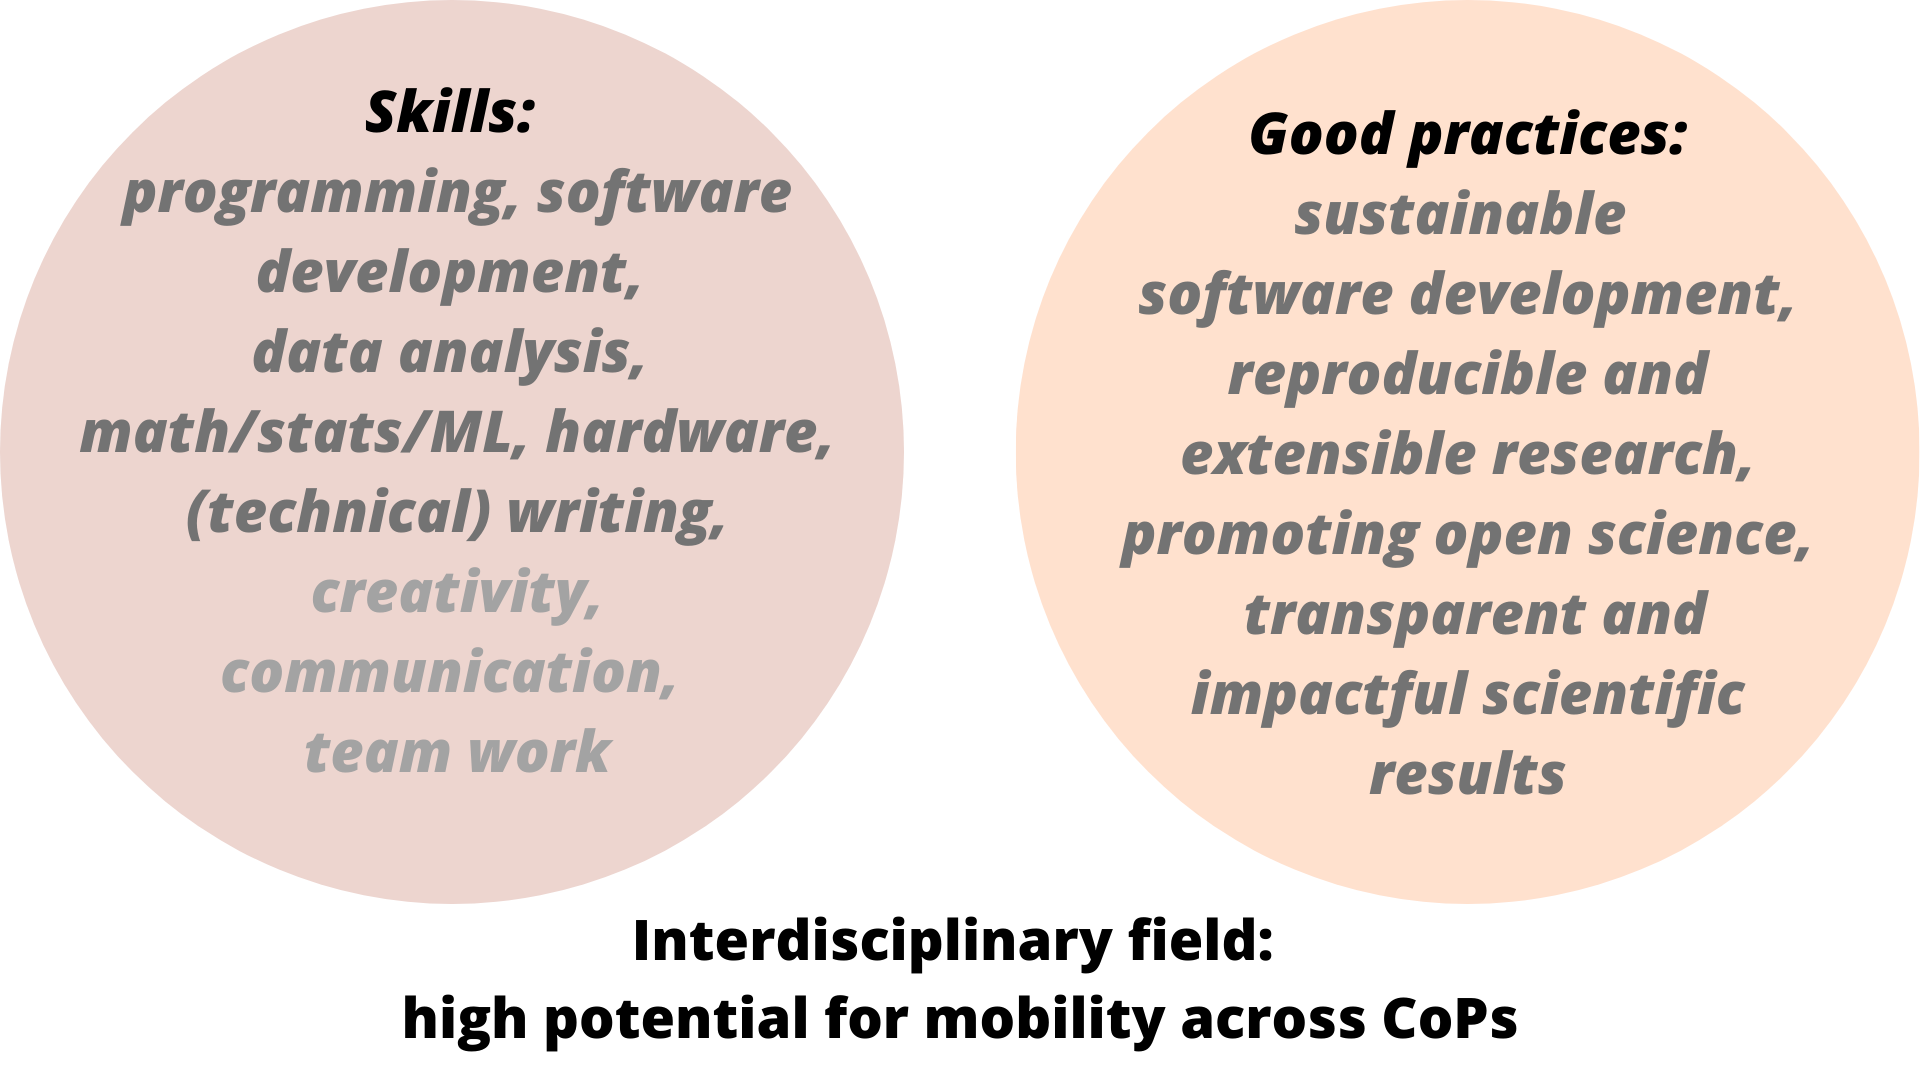
\includegraphics[width=1\textwidth,height=\textheight]{figs/4.png}
\end{frame}

\begin{frame}{Meetup groups}
\protect\hypertarget{meetup-groups}{}
An accessible format for CoPs in CompStat and data science:
\textbf{meetup groups}

\begin{itemize}
\item
  \href{https://meetup.com}{Meetup.com} is a platform for finding and
  building local communities
\item
  Regular events (online/in person) can be organized through the
  platform.
\end{itemize}

Tip: Many meetup groups organize joint events, so keep an eye for those
to discover new communities.
\end{frame}

\begin{frame}{Some relevant meetup groups}
\protect\hypertarget{some-relevant-meetup-groups}{}
\begin{itemize}
\item
  R User Local Groups (see also
  \href{https://www.r-consortium.org/all-projects/r-user-group-support-program}{R
  Consortium})
\item
  \href{https://rladies.org/}{R-Ladies}, a world-wide organization to
  promote gender diversity in the R community

  \begin{itemize}
  \tightlist
  \item
    offers an online directory of R-Ladies,
  \item
    global github repository
  \item
    supports local chapters who organize events
  \end{itemize}
\item
  \href{https://wiki.python.org/moin/LocalUserGroups}{Python User
  Groups}
\item
  \href{https://pyladies.com/}{PyLadies}, a global group with the focus
  on getting more women involved in the Python open-source community
\item
  \href{https://www.meetup.com/de-DE/pro/pydata/}{PyData Groups}
\item
  \href{https://www.meetup.com/de-DE/topics/julia/all/?all=1}{Julia
  Users Groups}
\item
  \href{https://discourse.julialang.org/t/announcing-julia-gender-inclusive/63702}{Julia
  Gender Inclusive}
\end{itemize}
\end{frame}

\begin{frame}{}
\protect\hypertarget{section}{}
\vspace{1em}
\begin{figure}
  \begin{columns}
    \begin{column}{.5\linewidth}
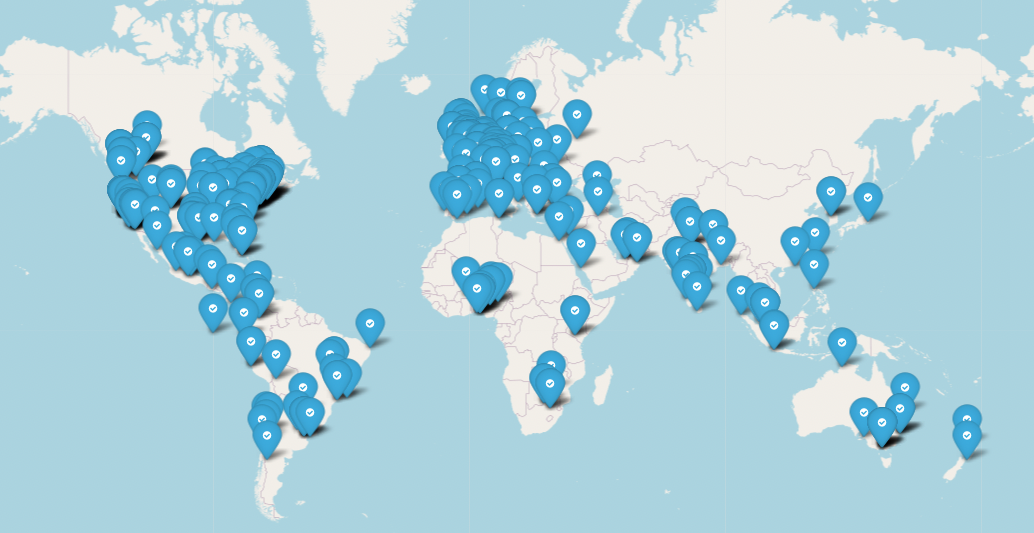
\includegraphics{figs/Rusergroups.png}
    \end{column}
    \begin{column}{.5\linewidth}
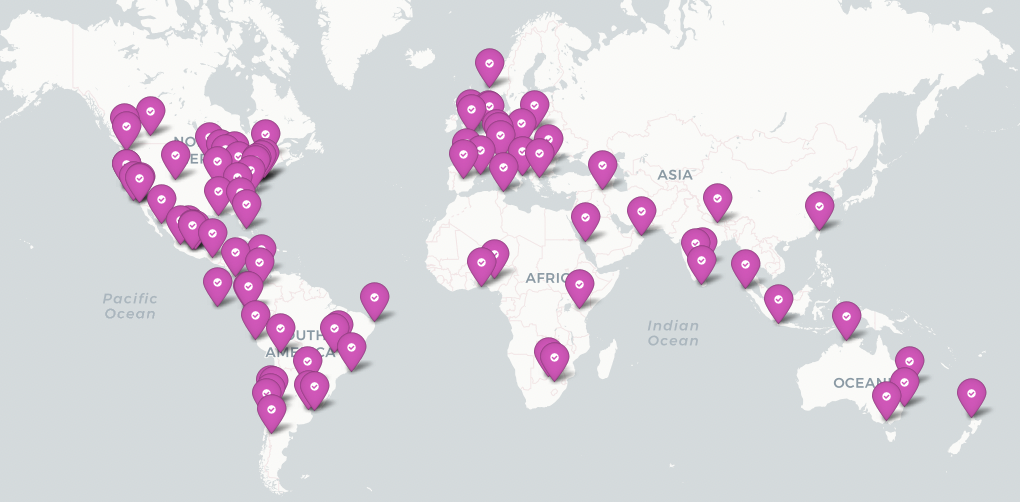
\includegraphics{figs/RLadiesgroups.png}
    \end{column}
      \end{columns}
    \caption{Active R User and R-Ladies Groups, \href{https://benubah.github.io/r-community-explorer/rugs.html}{Dashboard by Ben Ubah}}
    \end{figure}
\vspace{-3em}

\begin{figure}
\centering
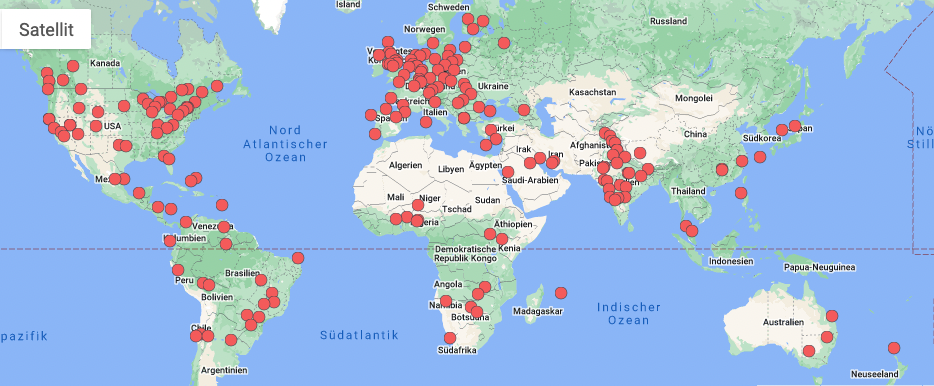
\includegraphics{figs/PyDatagroups.png}
\caption{PyData Groups}
\end{figure}
\end{frame}

\begin{frame}{Building inclusive CoPs \& events}
\protect\hypertarget{building-inclusive-cops-events}{}
\begin{figure}
\centering
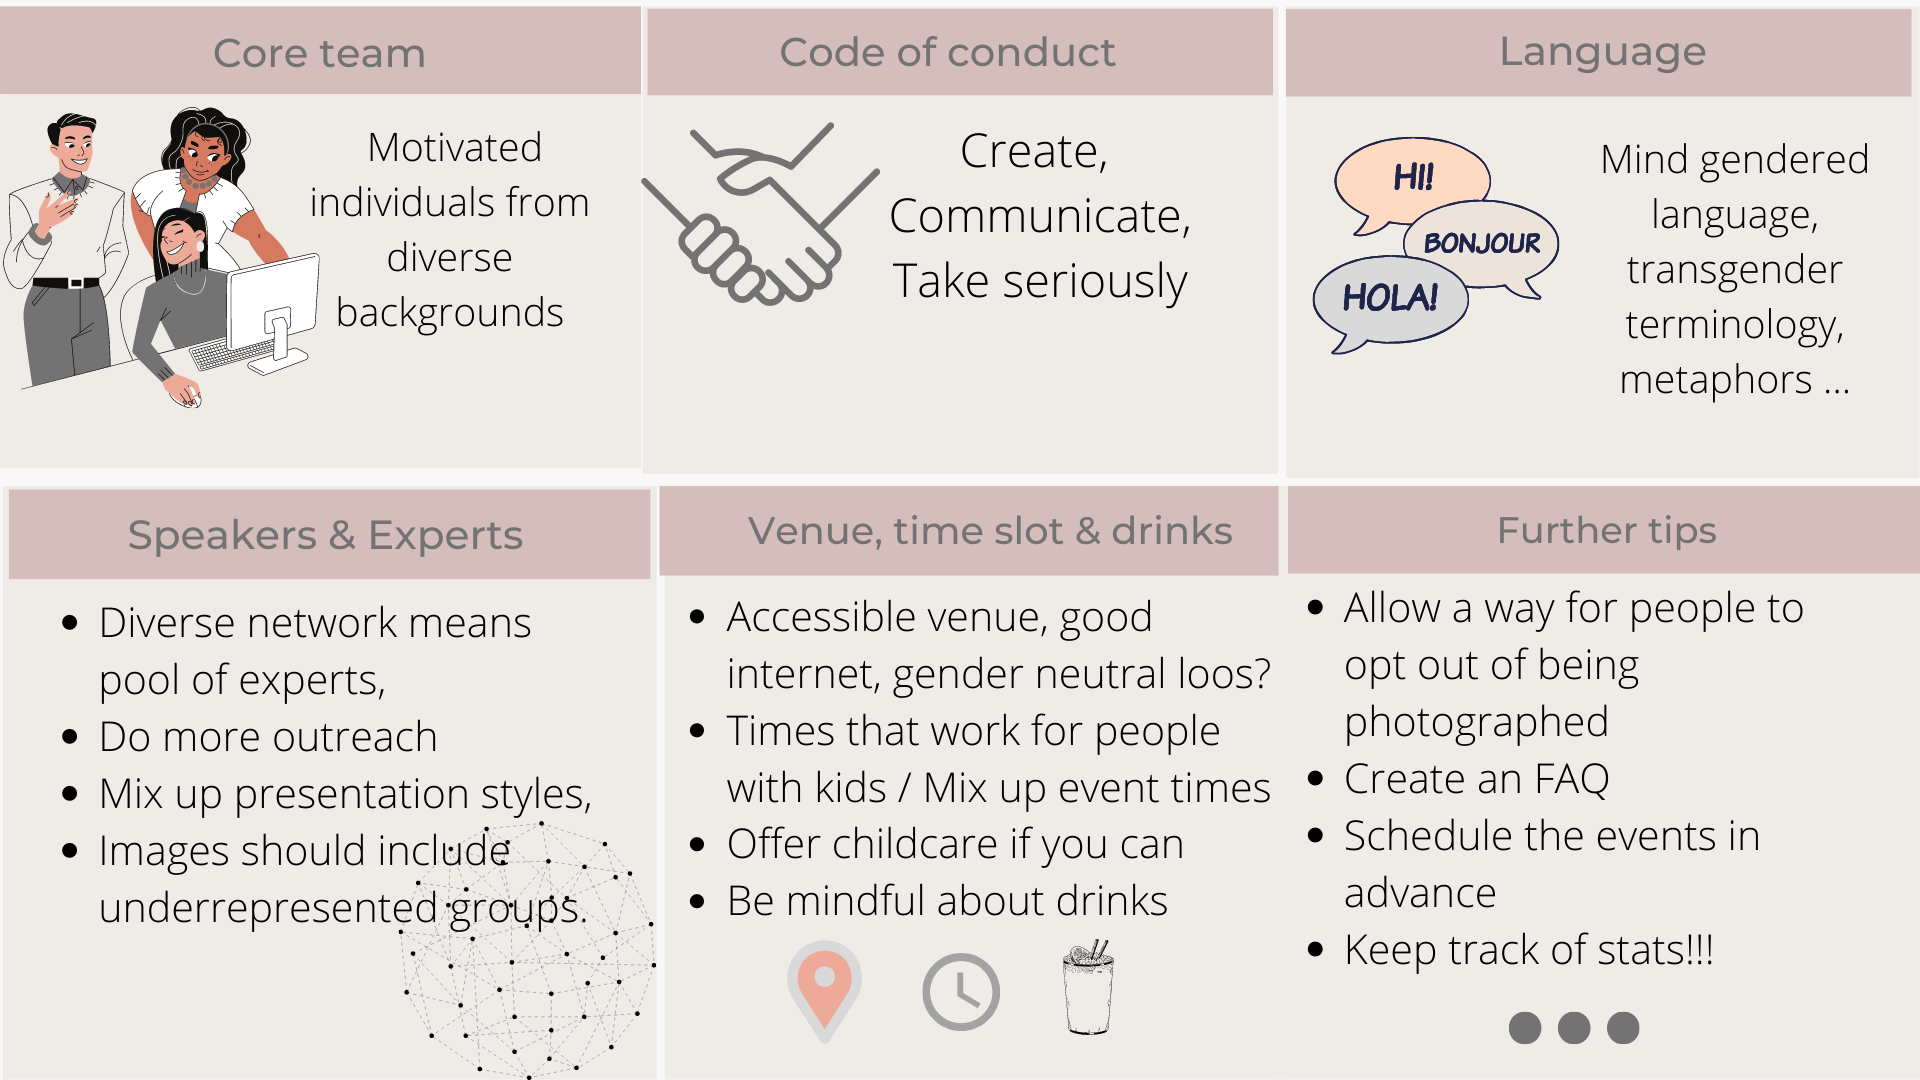
\includegraphics[width=1\textwidth,height=\textheight]{figs/2.png}
\caption{Inspired from
\href{https://make.wordpress.org/community/handbook/wordcamp-organizer/}{WordCamp
Organizer} and Andy Burgin on
\href{https://medium.com/@andyburgindevops/building-an-inclusive-and-diverse-tech-meetup-50efc5cf81e1}{Medium}}
\end{figure}
\end{frame}

\begin{frame}{Thank you!}
\protect\hypertarget{thank-you}{}
Laura Vana-Gür (TU Wien, R-Ladies Vienna Chapter)

Email:
\href{mailto:laura.vana.guer@tuwien.ac.at}{\nolinkurl{laura.vana.guer@tuwien.ac.at}}
\newline Github: \url{https://github.com/lauravana} \newline Twitter:
@llauriciu, @RLadiesVienna

Slides are available at: \url{https://github.com/lauravana/COMPSTAT2022}
\end{frame}

\begin{frame}{References}
\protect\hypertarget{references}{}
\hypertarget{refs}{}
\begin{CSLReferences}{1}{0}
\leavevmode\vadjust pre{\hypertarget{ref-brown1991organizational}{}}%
Brown, John Seely, and Paul Duguid. 1991. {``Organizational Learning and
Communities-of-Practice: Toward a Unified View of Working, Learning, and
Innovation.''} \emph{Organization Science} 2 (1): 40--57.
\url{https://doi.org/10.1287/orsc.2.1.40}.

\leavevmode\vadjust pre{\hypertarget{ref-constant1987social}{}}%
Constant II, Edward W. 1987. {``The Social Locus of Technological
Practice: Community, System, or Organization?''} In \emph{The Social
Construction of Technological Systems}, 223--42. Cambridge MA: MIT
Press.

\leavevmode\vadjust pre{\hypertarget{ref-erik2005archetypes}{}}%
Erik Andriessen, JH. 2005. {``Archetypes of Knowledge Communities.''} In
\emph{Communities and Technologies}, 191--213. Springer.

\leavevmode\vadjust pre{\hypertarget{ref-hoadley2012community}{}}%
Hoadley, Christopher. 2012. {``What Is a Community of Practice and How
Can We Support It?''} In \emph{Theoretical Foundations of Learning
Environments}, 286--99. Routledge.
\url{https://www.academia.edu/36699359/What_is_a_community_of_practice_and_how_can_we_support_it}.

\leavevmode\vadjust pre{\hypertarget{ref-hoadley2005using}{}}%
Hoadley, Christopher M, and Peter G Kilner. 2005. {``Using Technology to
Transform Communities of Practice into Knowledge-Building
Communities.''} \emph{ACM SIGGroup Bulletin} 25 (1): 31--40.

\leavevmode\vadjust pre{\hypertarget{ref-kilner2004con4}{}}%
Kilner, Pete. 2004. {``The Con4-p Model of Learning Design for
Professional Communities.''} In \emph{E-Learn: World Conference on
e-Learning in Corporate, Government, Healthcare, and Higher Education},
1307--11. Association for the Advancement of Computing in Education
(AACE).

\leavevmode\vadjust pre{\hypertarget{ref-lave1991situated}{}}%
Lave, Jean, and Etienne Wenger. 1991. \emph{Situated Learning:
Legitimate Peripheral Participation}. Cambridge university press.

\leavevmode\vadjust pre{\hypertarget{ref-orr1990sharing}{}}%
Orr, Julian E. 1990. {``Sharing Knowledge, Celebrating Identity:
Community Memory in a Service Culture.''} In \emph{Collective
Remembering}, 169--89. Sage Publications, Inc.

\leavevmode\vadjust pre{\hypertarget{ref-stevens2018building}{}}%
Stevens, Sarah LR, Mateusz Kuzak, Carlos Martinez, Aurelia Moser, Petra
Bleeker, and Marc Galland. 2018. {``Building a Local Community of
Practice in Scientific Programming for Life Scientists.''} \emph{PLoS
Biology} 16 (11): e2005561.

\leavevmode\vadjust pre{\hypertarget{ref-wenger2000communities}{}}%
Wenger, Etienne C, and William M Snyder. 2000. {``Communities of
Practice: The Organizational Frontier.''} \emph{Harvard Business Review}
78 (1): 139--46.
\url{http://www.psycholosphere.com/Communities\%20of\%20Practice\%20-20the\%20organizational\%20frontier\%20by\%20Wenger.pdf}.

\end{CSLReferences}
\end{frame}

\end{document}
